\chapter{Fundamentos técnicos}\label{cap:tecnologias}

En este capítulo se detallan los fundamentos técnicos detrás de las mejoras a BT Studio, es decir, todas las herramientas, tecnologías y librerías utilizadas para el desarrollo de estas. Dada la naturaleza de BT Studio, estas herramientas pertenecen únicamente al ámbito del software y están divididas generalmente en dos tipos: herramientas usadas para el desarrollo web y herramientas para el desarrollo robótico. La única excepción a esta separación es el lenguaje de programación Python, que se usa en ambos. 

\section{Lenguaje Python}

Python\footnote{\url{https://www.python.org/}} es un lenguaje de programación de alto nivel interpretado, orientado a objetos (aunque también permite programación funcional) y con semántica dinámica. Es utilizado en un gran número de aplicaciones, desde servidores web a inteligencia artificial. 
En de BT Studio se ha utilizado la versión 3.10.12. 

Entre sus características más destacadas podemos encontrar:

\begin{itemize}
    \item Sintaxis sencilla y legible que enfatiza la legibilidad y, por lo tanto, reduce el costo de mantenimiento del programa.
    \item \textit{Batteries included}\footnote{\url{https://peps.python.org/pep-0206/}}: contiene mucha funcionalidad adicional out-of-the-box incluida en su librería standard. Además, existen infinidad de librerías de terceros. 
    \item Su uso es gratuito y posee una licencia de código abierto. 
    \item \textit{Tipado dinámico}: no es necesario declarar el tipo de las variables al inicializarlas y este puede cambiar en función del valor de la variable en un determinado momento. También se pueden declarar los tipos para volverlo estricto.
    \item Es un lenguaje interpretado, por lo que no necesita compilar el código. Las sentencias del programa se ejecutan conforme se leen. 
\end{itemize}

Todas estas características conllevan un empeoramiento del rendimiento y consumo de memoria comparado con otros lenguajes como C, lo que restringe el tipo de sistemas que pueden usarlo. Esto en el caso de BT Studio no afecta, y además Python es requerido por los siguientes motivos:

\begin{itemize}
    \item El motor de ejecutor de árboles solo permite describir las acciones en Python.
    \item El Robotics Backend, entorno donde se ejecutan las aplicaciones, solo soporta Python. 
    \item El backend web de BT Studio utiliza el framework Django que usa Python. 
\end{itemize}

\section{Herramientas de desarrollo web}

Estas son las herramientas que han sido usadas para los cambios en el backend y el frontend web, así como en las que se basa BT Studio. Este primero tiene como función servir la página web del IDE y proveer distintos servicios a través de una API REST. El segundo sirve para mostrar la interfaz gráfica en el navegador e interaccionar con esta, pudiendo usar los servicios soportados por el backend.

Se recapitulan ahora las tecnologías más usadas en estas mejoras, así como la mención a varias librerías usadas en la sección de React.

\subsection{HTML}

HTML\footnote{\url{https://html.spec.whatwg.org/}} es un lenguaje de marcado estándar usado para definir la estructura de un documento web mediante etiquetas, que encapsulan las diferentes partes del contenido para darles una determinada apariencia o funcionalidad. Estos archivos no son ejecutables, si no que son leídos y representados por los navegadores web de forma transparente al usuario. 

Para este trabajo, se ha utilizado la última versión del \textit{living standard} de HTML\footnote{\url{https://developer.mozilla.org/en-US/docs/Glossary/HTML5}}. 

\subsection{CSS}

CSS\footnote{\url{https://www.w3.org/Style/CSS/}} es un lenguaje de hojas de estilo usado para especificar la presentación y el estilo de un documento escrito en un lenguaje de marcado como HTML o XML. El objetivo de CSS es permitir la separación de contenido y presentación, incluidos diseño, colores y fuentes en distintos ficheros, consiguiendo dividir la estructura, de la apariencia de la aplicación.

En BT Studio se ha usado la última versión disponible de CSS, 4.15.

\subsection{JavaScript}

JavaScript\footnote{\url{https://ecma-international.org/publications-and-standards/standards/ecma-262/}} es un lenguaje de programación de alto nivel interpretado, usado habitualmente para dotar de interactividad y dinamismo a las páginas web. Es un lenguaje no tipado, es decir, no se permite la definición del tipo de una variable. Junto con HTML y CSS forma el \textit{stack} básico en el desarrollo web.

En el desarrollo de este trabajo se empezó usando JavaScript, pero se acabó remplazando por TypeScript.

\begin{figure}[H]
    \centering
    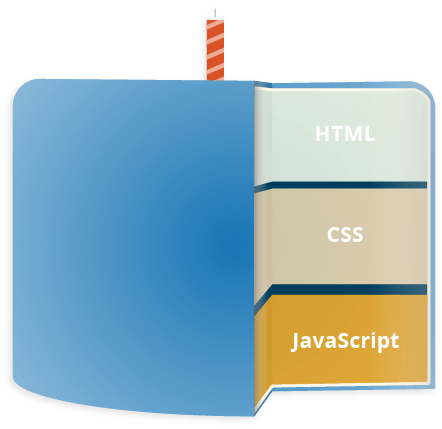
\includegraphics[width=0.3\textwidth]{figures/web_stack.png}
    \caption{Stack típico de desarrollo web}
    \label{fig:ejemplo}
\end{figure}

\subsection{TypeScript}
TypeScript\footnote{\url{https://www.typescriptlang.org}} es un lenguaje de programación de alto nivel basado en JavaScript, pero que cuenta con tipado estricto, es decir, se debe declarar el tipo de la variable al inicializarse y en todo lugar donde se pasen argumentos. Esto permite un mejor control del código, siendo completamente compatible con JavaScript

Concretamente, en el web IDE BT Studio se ha usado la versión 5.2.2 de TypeScript dentro de la librería REACT. 
\subsection{React}

React\footnote{\url{https://react.dev/reference/react}} es un \textit{framework} de JavaScript de código abierto diseñada para crear interfaces de usuario, especialmente en aplicaciones de una sola página. Es mantenida por Facebook y una comunidad de desarrolladores individuales y empresas. La versión empleada en este TFG fue la 18.2.0. 

Sus características más importantes son: 

\begin{itemize}
    \item \textbf{Componentes reutilizables}: permite la creación de interfaces de usuario a partir de piezas individuales llamados componentes. Estos mejoran la modularidad y escalabilidad de la aplicación.
    
    \item \textbf{Virtual DOM}: utiliza un DOM virtual que es una representación en memoria del DOM real con el objetivo de optimizar la actualización del este, actualizando solo las partes que han cambiado en cada momento, mejorando el rendimiento.
    
    \item \textbf{JSX o TSX}: introduce una sintaxis que permite escribir la estructura del componente de UI en código similar a HTML dentro de archivos JavaScript o TypeScript. Esto mejora la legibilidad del código y facilita el desarrollo. 
    
    \item \textbf{Flujo de datos unidireccional}: los datos solo se actualizan en un sentido, facilitando el rastreo de cambios a lo largo de la aplicación y mejora la predictibilidad y la facilidad de depuración.
    
    \item \textbf{Hooks}: son funciones que permiten a los componentes funcionales tener estado y acceder a características del ciclo de vida de React.
    
    \item \textbf{Ecosistema extenso}: al ser una librería de JavaScript existe un amplio ecosistema de herramientas, bibliotecas y frameworks compatibles con React.
\end{itemize}

React se ha utilizado para la creación de nuevos componentes en el frontend de BT Studio, así como en los ya existentes.

Algunas de las librerías compatibles con React más importantes durante el desarrollo de las mejoras han sido:

\begin{itemize}
    \item \textbf{Projectstorm React Diagrams}: usado tanto en el editor de árboles de comportamiento como en el monitor de ejecución. Más detalles de su uso en BT Studio, se pueden encontrar en este TFG \cite{TFG_BT_Studio}.
    \item \textbf{Monaco Editor\footnote{\url{https://microsoft.github.io/monaco-editor/}}}: usado para sustituir al antiguo editor ACE. Esta librería está mantenida por Microsoft bajo la licencia de código abierto MIT y proporciona un editor con toda la funcionalidad del usado en VS Code.
\end{itemize}

\subsection{Webpack}

Webpack\footnote{\url{https://webpack.js.org}} es una herramienta de código abierto usada para empaquetar aplicaciones de JavaScript junto con recursos del frontend como HTML, CSS o imágenes usando cargadores configurables.

En este TFG se ha usado Webpack en la integración de BT Studio en Unibotics y en la dockerización de la ejecución del primero.   

\subsection{Django}

Django\footnote{\url{https://www.djangoproject.com/}} es un \textit{framework} de desarrollo web de código abierto, gratuito y escrito en Python. Proporciona una estructura de organización específica siguiendo la filosofía de reducir la redundancia de código, lo que facilita la creación aplicaciones web complejas y robustas de manera eficiente. Para el desarrollo de BT Studio se ha utilizado la versión LTS, Django 4.2. 

\noindent Las características más importantes de Django en su uso en BT Studio son:

\begin{itemize}
    % \item \textbf{Rapidez}: fue diseñado para crear aplicaciones web lo más rápido posible. Esto implica que tiene un diseño claro, bien estructurado y con una gran variedad de funcionalidades y herramientas adicionales. 
    
    \item \textbf{Seguridad}: incluye herramientas para evitar los problemas comunes de seguridad, como los ataques XSS, el CSRF o la inyección SQL. Además, soporta de manera completa el protocolo HTTPS. Esto era necesario para permitir una integración en Unibotics segura. 
    
    % \item \textbf{Escalable}: una vez implementada una funcionalidad en Django, esta puede ser usada desde el nivel de prototipo hasta el despliegue en aplicación web con miles de usuarios con cambios mínimos. Esto lo consigue mediante herramientas como cachés o la división de bases de datos en particiones. 
    
    \item \textbf{Plantillas}: son archivos HTML enriquecidos con marcadores y etiquetas especiales de Django, que permiten la generación dinámica de la apariencia de la interfaz. 
    
    \item \textbf{Patrón modelo-vista-controlador}: es un patrón de diseño de software usado comúnmente para la implementación de interfaces y su lógica de control. Esto permite separar la lógica de la visualización. 
    \begin{itemize}
        \item \textit{Modelo}: representa los datos necesarios para una determinada aplicación y la estructura de la base de datos. 
        \item \textit{Vista}: define cómo se muestran los datos de la aplicación, así como la interfaz para realizar operaciones sobre ellos. 
        \item \textit{Controlador}: contiene la lógica para actualizar los modelos y las vistas en respuesta a las acciones de los usuarios. 
    \end{itemize}

    \item \textbf{Fácil mantenimiento}: al utilizar el patrón MVC y plantillas, la estructura resultante es modular y fácilmente reutilizable.
    
\end{itemize}

\begin{figure}[htp]
    \centering
    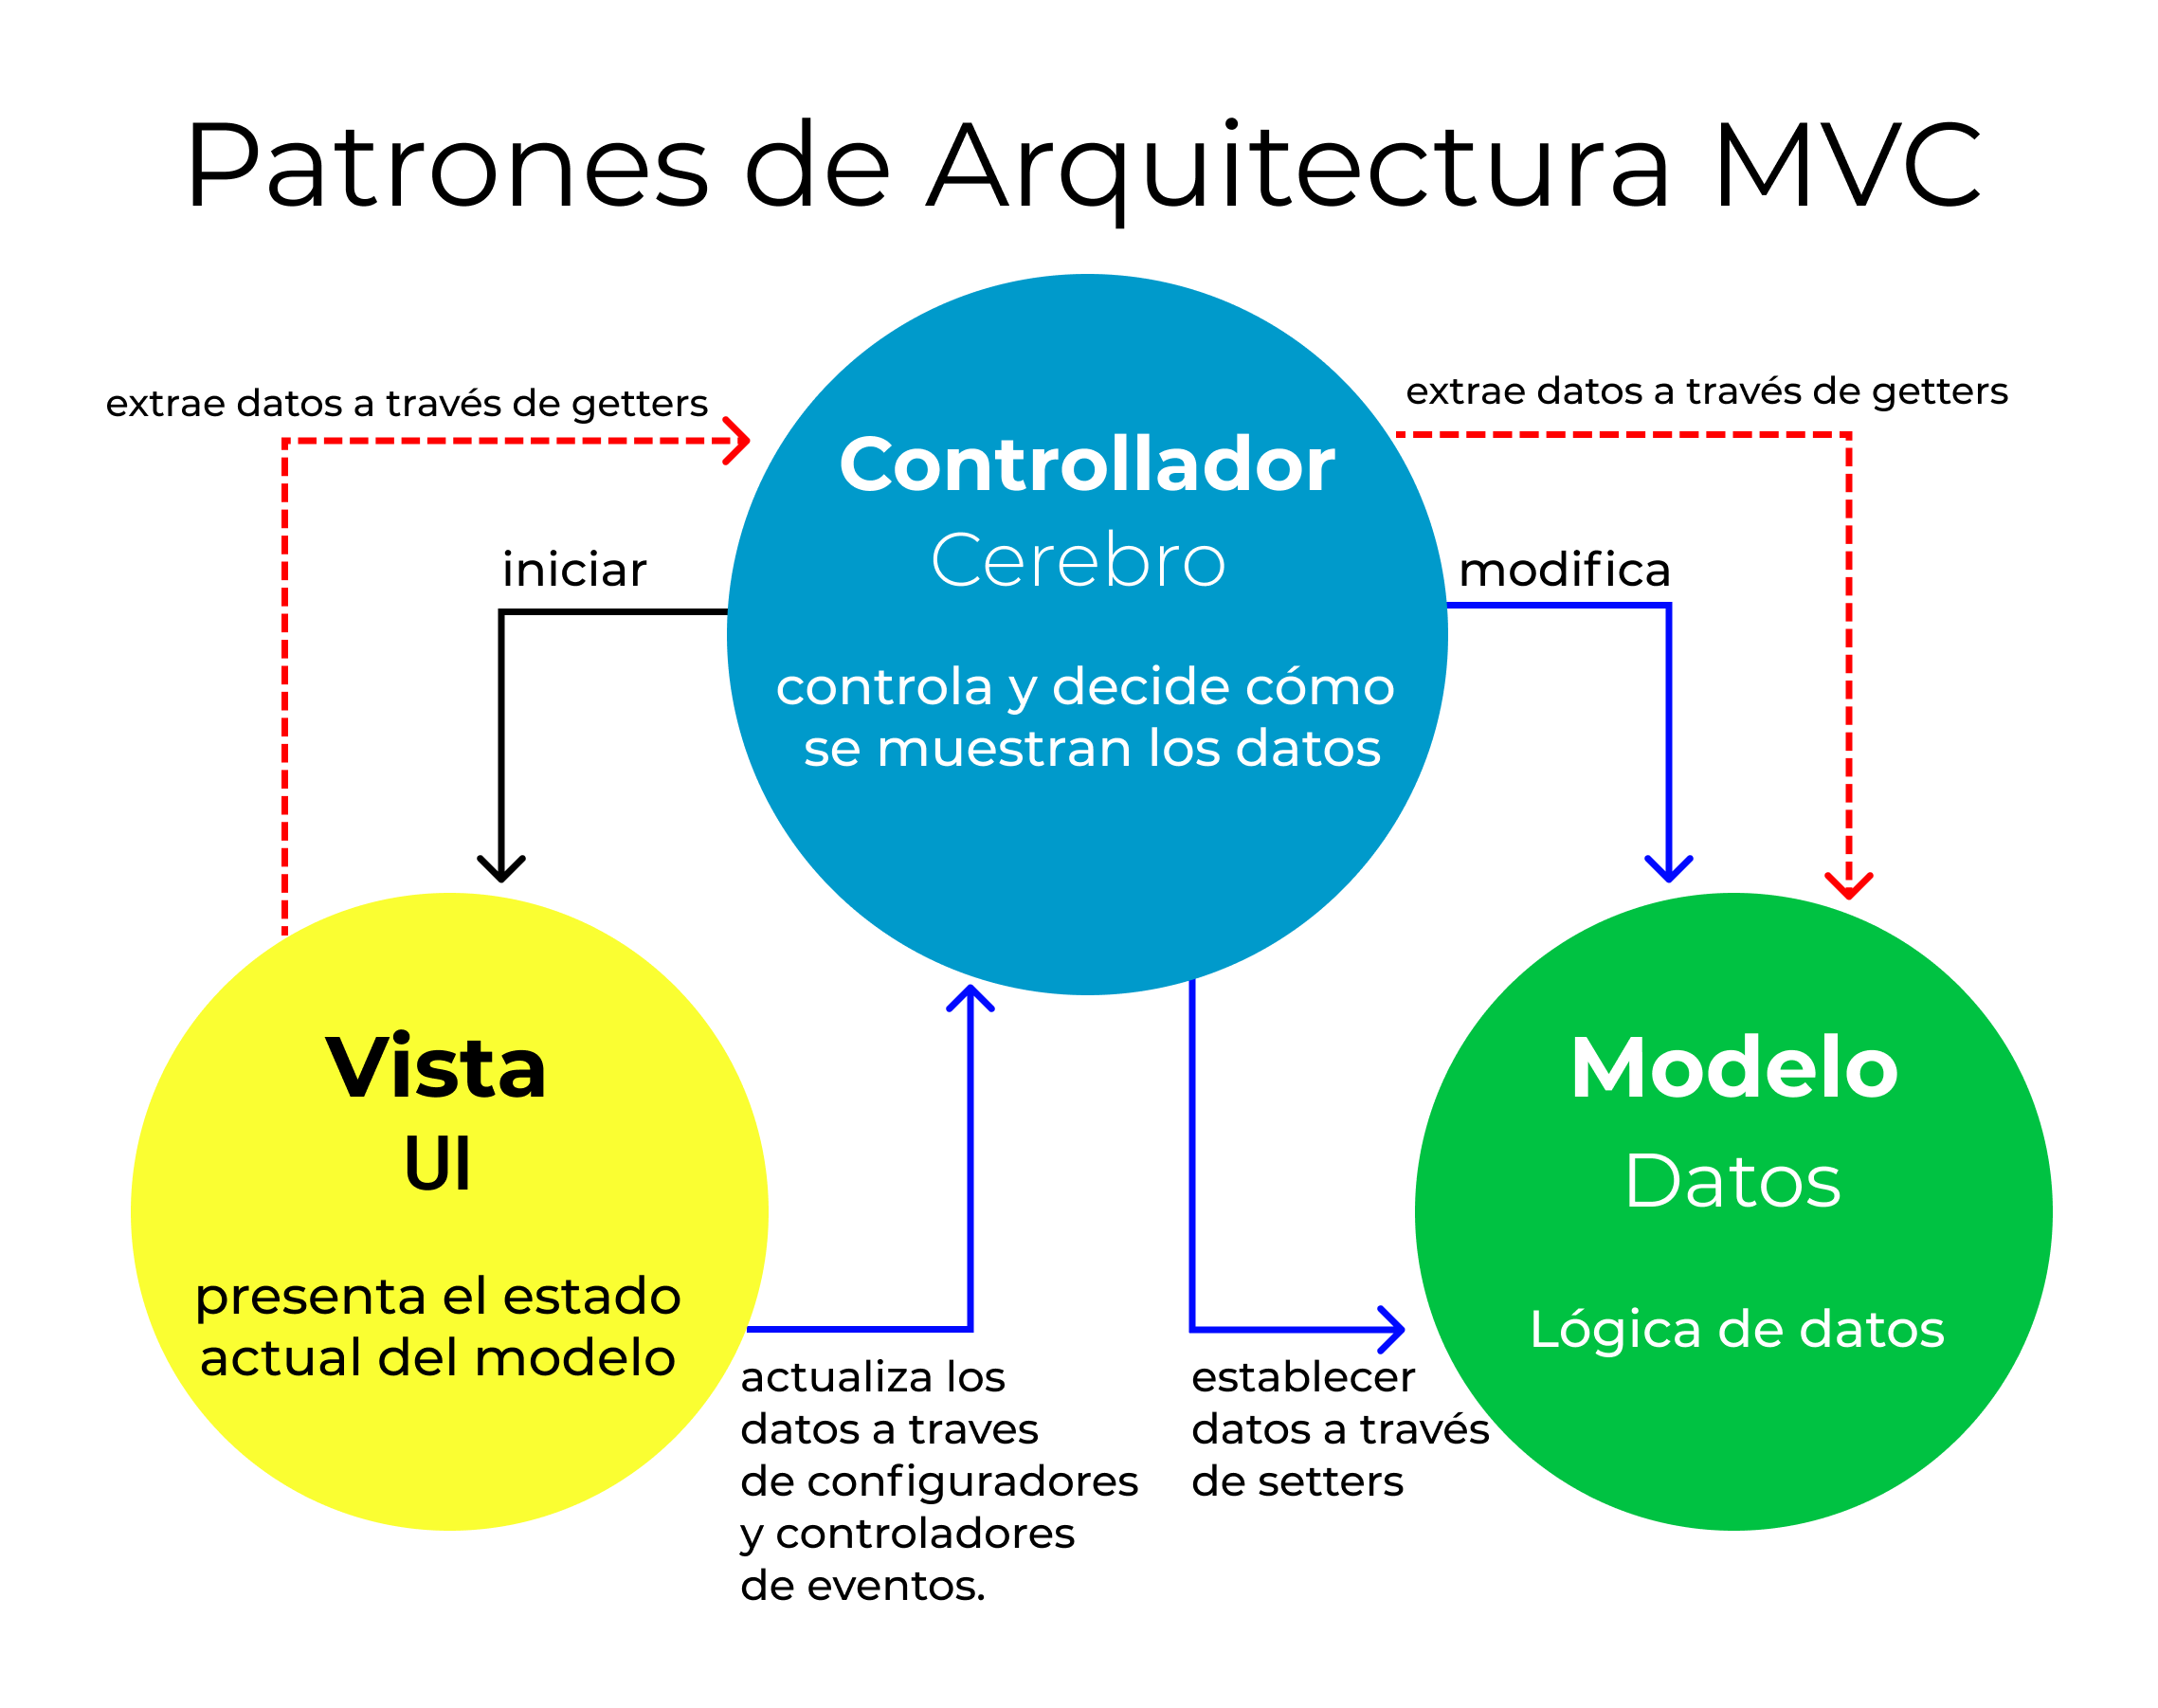
\includegraphics[width=0.6\textwidth]{figures/mvc.png}
    \caption{Esquema Modelo-Vista-Controlador}
    \label{fig:ejemplo}
\end{figure}

\subsection{WebSocket}

WebSocket\footnote{\url{https://www.rfc-editor.org/rfc/rfc6455}} es un protocolo de comunicación full-duplex sobre una única conexión TCP. Este protocolo tiene como objetivo el facilitar la interacción en tiempo real entre el cliente y el servidor, siendo fundamental para aplicaciones que requieren una comunicación bidireccional persistente y con baja latencia. En BT Studio, son usados para la comunicación entre el web IDE y el entorno de ejecución dockerizado. 

Las características más importantes de este protocolo son las siguientes:

\begin{itemize}
    \item \textbf{Comunicación Full-Duplex:} permite que tanto el cliente como el servidor envíen datos simultáneamente y en cualquier momento. Esto mejora la interactividad y el rendimiento de las aplicaciones al eliminar la necesidad de realizar múltiples conexiones HTTP para la comunicación.
    
    \item \textbf{Sesión persistente:} a diferencia del modelo de solicitud-respuesta utilizado en HTTP, WebSockets establece una conexión persistente que permanece abierta hasta que el cliente o el servidor desee.
    
    \item \textbf{Menor sobrecarga:} tras el establecimiento inicial de la conexión, la sobrecarga de datos es significativamente menor en comparación con HTTP, ya que los encabezados no necesitan ser enviados junto a cada mensaje.
    
    \item \textbf{Compatibilidad con navegadores:} el protocolo está soportado por todos los navegadores modernos.
    
    \item \textbf{Facilidad de uso:} la API de WebSockets es simple y fácil de usar, permitiendo establecer una comunicación bidireccional cliente-servidor con pocas líneas de código.
\end{itemize}

\subsection{VNC en la web}

Virtual Network Computing\footnote{\url{https://quentinsf.com/publications/virtual-network-computing/vnc-ieee.pdf}} es un sistema que permite la visualización y control remoto de una máquina, servidor, desde otra, cliente. En BT Studio se utiliza para transmitir la interfaz gráfica del simulador y el terminal que se encuentran dentro del docker del Robotics Backend, así como para permitir la interacción con ambas desde el frontend del web IDE donde se hallan dos clientes de VNC.

Las características fundamentales de VNC en una implementación web incluyen:

\begin{itemize}
    \item \textbf{Seguridad:} las implementaciones web de VNC pueden usar protocolos de seguridad como TLS/SSL para cifrar la conexión entre el navegador y el servidor VNC. 
    
    \item \textbf{Navegador como cliente VNC:} utilizando otras tecnologías web como HTML y WebSockets, es posible la implementación del sistema VNC en los navegadores. Esto permite a los usuarios controlar sistemas remotos directamente desde el navegador sin necesidad de instalar clientes de VNC en su propio sistema. Esto permite la interoperabilidad entre sistemas operativos. 
    
    \item \textbf{Interactividad:} gracias al uso de WebSockets para una comunicación bidireccional eficiente, las implementaciones web de VNC ofrecen interactividad con una mínima latencia. Esto resulta fundamental para BT Studio debido a que por naturaleza las simulaciones robóticas son muy reactivas. 
\end{itemize}

\section{Herramientas de desarrollo robótico}

\subsection{ROS 2}
\label{ros_2}

ROS 2\footnote{\url{https://docs.ros.org/en/humble/index.html}} (Robot Operating System 2) es un conjunto de librerías y herramientas para el desarrollo de aplicaciones robóticas. Este además incluye una extensa colección de drivers y algoritmos del estado del arte. Se puede consultar su diseño en profundidad en \cite{Macenski_2022}. La versión utilizada en este TFG es la última versión LTS disponible a su comienzo, Humble Hawksbill. 

Las aplicaciones que se generan en BT Studio son aplicaciones ROS 2, con un nodo que posee la capacidad de interactuar con los drivers de los sensores y actuadores del robot usando una interfaz llamada \textit{topic}. 

Las características que definen el diseño de ROS 2 son las siguientes:

\begin{itemize}
    \item \textbf{Arquitectura distribuida:} utiliza un modelo de comunicación basado en DDS (Data Distribution Service) para la comunicación entre componentes en el sistema. Esto permite además el uso de políticas de calidades de servicio que garantizan unos requisitos concretos a las comunicaciones. 

    \item \textbf{Flexibilidad en la comunicación:} soporta múltiples patrones de comunicación, como publicador/suscriptor, servicios y acciones.

    \item \textbf{API homogénea en Python y C++}: la funcionalidad de ROS 2 se encuentra en la librería \textbf{rcl}, escrita en C. A partir de esta, se proporcionan APIs en lenguajes de alto nivel a través de librerías clientes, como \texttt{rclcpp} para C++ y \texttt{rclpy} para Python, que pueden ser usadas de manera simultánea para distintos componentes dentro de una misma aplicación robótica. 

    \item \textbf{Herramientas de desarrollo y depuración:} proporciona un extenso conjunto de herramientas para la depuración y visualización de sistemas robóticos, como Rviz2, para facilitar el desarrollo y la prueba de aplicaciones robóticas.
    
    \item \textbf{Soporte multiplataforma:} ROS 2 es compatible con varios sistemas operativos, incluyendo Linux (Ubuntu y RHEL), Mac OS, Windows y otros sistemas operativos en tiempo real, extendiendo así su uso en entornos robóticos diversos.
\end{itemize}

Con todas estas características podemos definir ROS 2 de manera más exacta como un \textit{middleware} que utiliza un mecanismo de publicador/subscriptor anónimo para la comunicación usando mensajes tipados entre distintos procesos o nodos. 

\subsubsection{Componentes básicos}

Por último, los componentes funcionales básicos que forman parte de ROS 2 son los siguientes:

\begin{itemize}
    \item \textbf{Nodos}: unidad de computación básica dentro del grafo de ROS. Usan una librería cliente (\textit{rclpy} o \textit{rclcpp}) para comunicarse con otros nodos que pueden estar en el mismo proceso, en otros o incluso en una máquina distinta.

    \item \textbf{Topics}: permiten conectar productores (publicadores) de datos con consumidores (subscriptores) a través de un canal de nombre común (topic). Además, poseen distintas calidades de servicio para la recepción de estos mensajes.

    \item \textbf{Interfaces:} definen las estructuras de los mensajes intercambiados entre los nodos mediante un lenguaje de definición de interfaces simplificado (IDL). 

    \item \textbf{Servicios:} son llamadas a procedimientos remotos, es decir, un nodo cliente puede invocar la ejecución de tareas y obtener un resultado por parte de un nodo servidor. Estos son normalmente de corta duración debido a que son bloqueantes para el nodo cliente. Si tienen una duración mayor se usan acciones.
    
    \item \textbf{Acciones:} son llamadas a procedimientos remotos de larga duración. Las acciones proporcionan \textit{feedback} mientras se están ejecutando y pueden ser canceladas en cualquier momento. 

    \item \textbf{Parámetros:} permiten la configuración de los nodos al iniciarse o en tiempo de ejecución sin cambios en el código fuente. En ROS 2, los parámetros están asociados a cada nodo y estos deben declarar todos los parámetros que aceptan junto con su tipo. 

    \item \textbf{Launch system:} tiene como objetivo automatizar el lanzamiento de múltiples nodos desde un solo comando. Permite definir cómo y cuándo ejecutar cada programa con una sintaxis común de ROS que facilita su reutilización. Esta sintaxis suele estar en Python, XML o YAML.
    
    \item \textbf{Descubrimiento de nodos}: es llevado a cabo de manera automática por el \textit{middleware} encargado de las comunicaciones en ROS2. Esto permite modificar el grafo añadiendo o eliminando nodos que pertenezcan al dominio de ROS de la aplicación.
    
\end{itemize}

\subsection{Simulador Gazebo}
\label{gazebo}

Gazebo\footnote{\url{https://gazebosim.org/home}} es un simulador 3D de código abierto mantenido por la Open Source Robotics Foundation utilizado ampliamente en el desarrollo de sistemas robóticos, específicamente en ROS2. Ofrece la capacidad de simular con precisión el funcionamiento de robots en entornos complejos y dinámicos. En BT Studio, más concretamente en el entorno de ejecución dockerizada Robotics Backend, se usa la última versión de Gazebo Classic, Gazebo 11, y la moderna, Gazebo Harmonic. 

Sus características más importantes son:

\begin{itemize}
    \item \textbf{Simulación realista:} utiliza motores de física avanzados como ODE (Open Dynamics Engine), Bullet o DART para proporcionar una simulación adecuada de fuerzas, colisiones y materiales. Esto permite simular robots y sistemas de control en entornos seguros y controlados que se asemejan al mundo real. 
    
    \item \textbf{Entornos ricos y personalizables:} permite la creación de entornos detallados con una amplia gama de objetos, texturas y condiciones de iluminación. Estos entornos son definidos en el formato SDF\footnote{\url{http://sdformat.org/}}, basado en XML. 
    
    \item \textbf{Librerías de sensores y actuadores:} proporciona una amplia variedad de modelos de sensores y actuadores que imitan de manera realista el comportamiento y las limitaciones de los modelos reales.
    
    \item \textbf{Interfaz gráfica y herramientas de usuario:} permite visualizar y manipular las simulaciones de manera gráfica, incluyendo la capacidad de controlar el tiempo de simulación, visualizar datos de sensores y editar en tiempo real objetos y entornos.
    
    \item \textbf{Integración con ROS 2:} se integra de manera completa con ROS 2, permitiendo a la aplicación de ROS 2 interactuar con la simulación como si fuera hardware real. 
\end{itemize}

\begin{figure}[H]
    \centering
    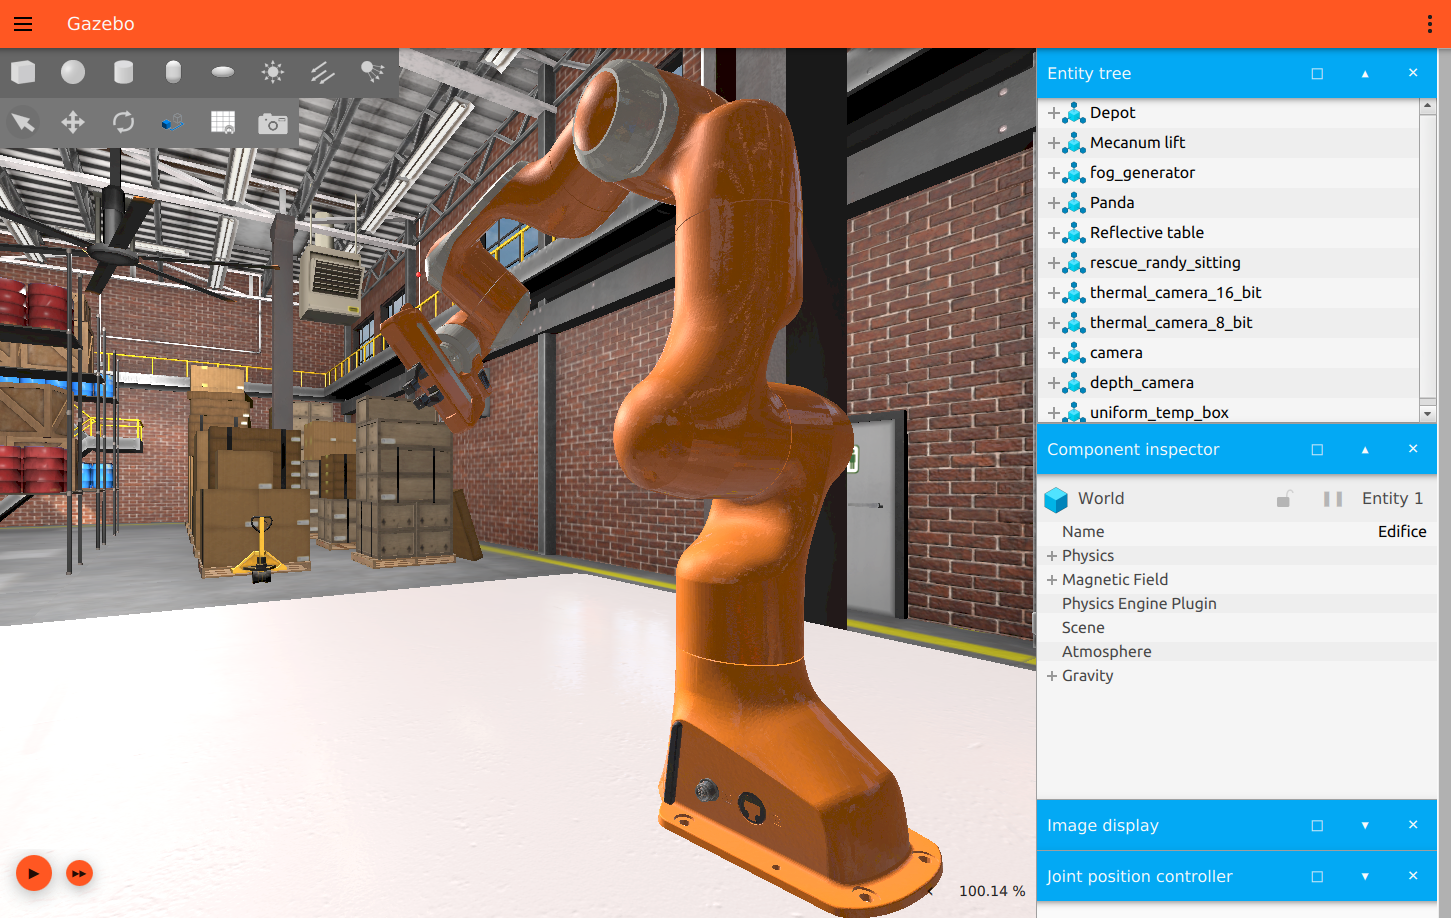
\includegraphics[width=0.8\textwidth]{figures/fundamentos/harmonic.png}
    \caption{Cliente gráfico de Gazebo Harmonic}
    \label{fig:ejemplo}
\end{figure}

\subsection{Árboles de comportamiento}

En esta sección se va a hablar de forma resumida sobre las características básicas de los árboles de comportamiento y de la librería PyTrees. Para una explicación más detallada sobre estos, BT.cpp y su uso en BT Studio se recomienda leer el TFG \cite{TFG_BT_Studio}.

\subsubsection{Definición}

Los árboles de comportamiento\cite{Colledanchise_2018} constituyen una manera de organizar la forma en la que un agente autónomo, ya sea un robot o una entidad virtual en un videojuego, alterna entre diferentes acciones. Para que una aplicación pueda usar este paradigma se necesita dividirla en distintos nodos reutilizables llamados acciones o nodos de control. Gracias a esto se consigue construir sistemas complejos que son al mismo tiempo modulares y reactivos.

\begin{figure}[H]
    \centering
    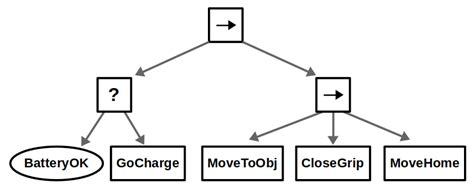
\includegraphics[width=0.8\textwidth]{figures/fundamentos/bt-example.png}
    \caption{Ejemplo básico de árbol de comportamiento}
    \label{fig:ejemplo}
\end{figure}

\subsubsection{Características}

Podemos entender la estructura de un árbol de comportamiento como la combinación de tres partes:

\begin{itemize}
    \item \textbf{Nodo raíz}: solo existe uno y es el origen del árbol de comportamiento. No tiene ningún nodo padre.
    \item \textbf{Nodos internos}: pueden existir cualquier número de estos y son los encargados de controlar el flujo de la ejecución. También son llamados nodos de control y poseen tanto un nodo padre como un número indefinido de nodos hijos.
    \item \textbf{Nodos externos}: pueden existir cualquier número de estos y son las acciones definidas por el usuario. Por esto también reciben el nombre de nodos de ejecución. Solo tienen un nodo padre.
\end{itemize}

La ejecución de un árbol de comportamiento empieza en el nodo raíz y se propagan a sus hijos usando señales a una determinada frecuencia llamadas \textit{ticks}. Cuando una de estas señales llega a un nodo hijo, este se ejecuta y devuelve uno de los siguientes estados: \textit{Running} si están ejecutando una tarea, \textit{Success} si ha conseguido su objetivo o \textit{Failure} en caso contrario. 

En la definición tradicional de los árboles de comportamientos, existen solo cuatro nodos de control de flujo (\textit{Sequence}, \textit{Fallback}, \textit{Parallel} y \textit{Decorator}) y dos de nodos de ejecución (\textit{Action} y \textit{Condition}). En BT.cpp\footnote{\url{https://github.com/BehaviorTree/BehaviorTree.CPP}}, la implementación de árboles de comportamiento en ROS 2, existen más nodos de control, pero no son importantes para este trabajo.

\noindent Funcionamiento de los nodos de control de flujo:

\begin{itemize}
    \item \textbf{Sequence:} ejecuta de manera secuencial sus hijos en el orden indicado hasta que uno devuelve \textit{Running} o \textit{Failure}. El nodo de control devolverá estos estados si esto ocurre o devolverá \textit{Success} si y sólo si todos los hijos lo devuelven.

    \begin{figure}[H]
        \centering
        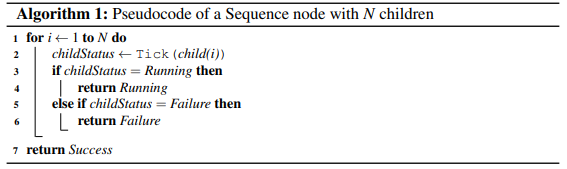
\includegraphics[width=0.8\textwidth]{figures/fundamentos/alg1.png}
        \caption{Algoritmo de un nodo tipo \textit{Sequence}}
        \label{fig:sequence}
    \end{figure}

    \item \textbf{Fallback:} ejecuta de manera secuencial sus hijos en el orden indicado hasta que uno devuelve \textit{Running} o \textit{Success}. El nodo de control devolverá estos estados si esto ocurre o devolverá \textit{Failure} si y sólo si todos los hijos lo devuelven.

    \begin{figure}[H]
        \centering
        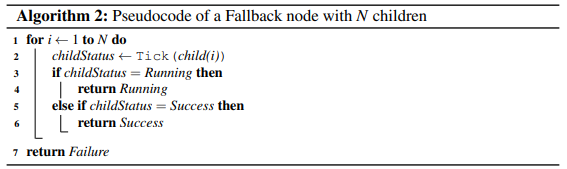
\includegraphics[width=0.8\textwidth]{figures/fundamentos/alg2.png}
        \caption{Algoritmo de un nodo tipo \textit{Fallback}}
        \label{fig:fallback}
    \end{figure}

    \item \textbf{Parallel:} ejecuta de manera paralela sus hijos y devolverá \textit{Success} si M hijos devuelven \textit{Success}, \textit{Failure} si N - M + 1 hijos devuelven \textit{Failure} y \textit{Running} en cualquier otro caso, siendo N es el número de hijos y M un umbral definido por el usuario.

    \begin{figure}[H]
        \centering
        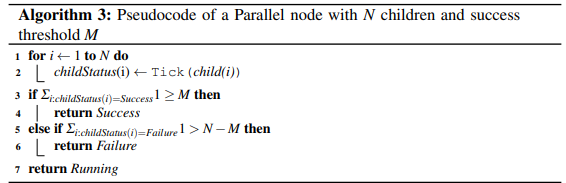
\includegraphics[width=0.8\textwidth]{figures/fundamentos/alg3.png}
        \caption{Algoritmo de un nodo tipo \textit{Parallel}}
        \label{fig:parallel}
    \end{figure}

    \item \textbf{Decorator:} son nodos de control que solo tienen un único hijo y manipulan el estado es la salida de este. Un ejemplo de este tipo es el nodo de control \textit{invert} que invierte la salida del hijo.

    \begin{figure}[H]
        \centering
        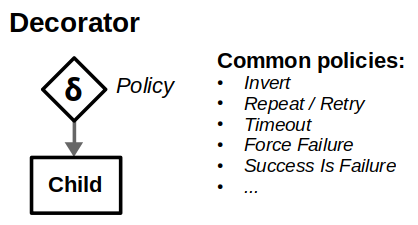
\includegraphics[width=0.4\textwidth]{figures/fundamentos/bt-decorator.png}
        \caption{Estructura de un nodo tipo \textit{Decorator}}
        \label{fig:parallel}
    \end{figure}
    
\end{itemize}

\noindent Funcionamiento de los nodos de ejecución:

\begin{itemize}
    \item \textbf{Action:} al recibir un tick, ejecutan una acción y devuelven \textit{Success} si ha tenido éxito, \textit{Failure} en caso contrario y \textit{Running} mientras está en ejecución. 

    \item \textbf{Condition:} al recibir un tick, comprueba una proposición y devuelve \textit{Success} o \textit{Failure} en función de su cumplimiento. Estos nodos nunca pueden devolver \textit{Running}.
    
\end{itemize}

\begin{figure}[H]
    \centering
    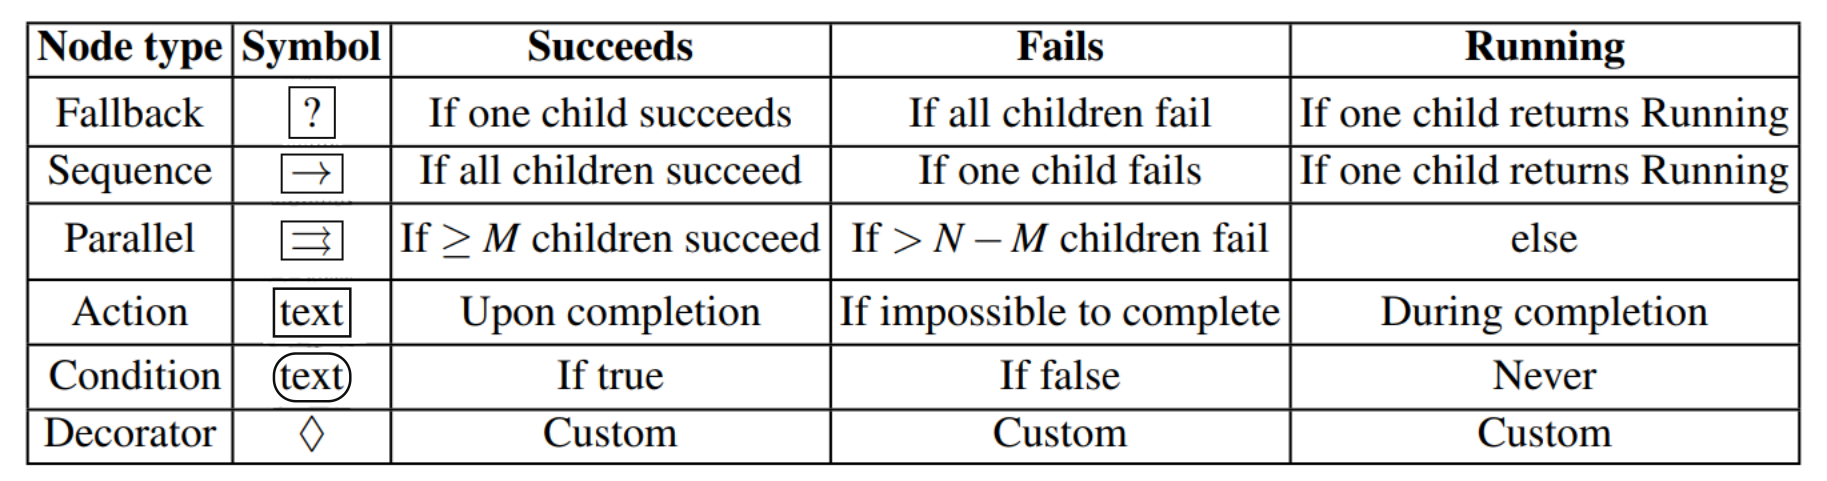
\includegraphics[width=\textwidth]{figures/fundamentos/node_types.png}
    \caption{Funcionamiento de los nodos de un árbol de comportamiento tradicional}
    \label{fig:ejemplo2}
\end{figure}

\subsubsection{PyTrees} \label{sec:blackboard}

PyTrees\footnote{\url{https://github.com/splintered-reality/py_trees}} es una librería para el desarrollo de árboles de comportamiento en Python en ROS 2. En BT Studio se usa la versión 2.3.0.

La característica que más importa para el desarrollo de este trabajo es la capacidad de extraer el estado del árbol de comportamiento en ejecución. Para una explicación más detallada sobre esta librería y su uso en BT Studio se recomienda la lectura del TFG \cite{TFG_BT_Studio}.

La extracción de este estado es posible gracias a las múltiple funciones encontradas en la sección de visualización de PyTrees, entre las que se encuentran:

\begin{itemize}
    \item \textbf{\textit{py\_trees.display.ascii\_tree()}}: devuelve el estado del árbol de comportamiento usando caracteres ASCII.
    \item \textbf{\textit{py\_trees.display.ascii\_blackboard()}}: devuelve el contenido de la \textit{blackboard} usando caracteres ASCII. La \textit{blackboard} es una memoria compartida que actúa como un diccionario de datos accesible por todos los nodos del árbol y permite la comunicación y el intercambio de información entre nodos mediante puertos.
\end{itemize}

A estas funciones es necesario pasarle como argumentos el árbol de comportamiento, pero como este ya era definido usando esta librería en BT Studio, no ha hecho falta utilizarla más que para lo indicado anteriormente.

% \subsubsection{Definición de nodos de ejecución}

% En PyTrees, los nodos de ejecución reciben el nombre de \textit{Behaviour} y no existe una separación explícita entre acciones y condiciones. Todos los comportamientos se implementan como una subclase de una clase base, donde se definen los siguientes métodos:

% \begin{itemize}

%     \item \textbf{\_\_init\_\_(name)}: inicialización mínima de la clase con la información necesaria para la introspección de los árboles mediante herramientas de depuración offline. 
    
%     \item \textbf{setup()}: método para inicialización diferida que se debe llamar manualmente o a través de métodos de la librería que configuran el comportamiento junto con sus descendientes. Adecuado para inicialización de hardware, middleware o cualquier configuración necesaria que no se desee en el constructor por interferir con la representación del árbol en gráficos o validaciones.
    
%     \item \textbf{initialise()}: invocado siempre que el estado anterior del comportamiento no sea \textit{RUNNING}. Aquí se realiza cualquier preparación requerida antes de comenzar la ejecución de una iteración del comportamiento. 
    
%     \item \textbf{update()}: este método se llama en cada tick del comportamiento. Dentro de este, se debe implementar la lógica principal del comportamiento, incluyendo decisiones, monitoreo o cualquier acción no bloqueante. Debe retornar un estado de \textit{py\_trees.common.Status}, que puede ser \textit{RUNNING}, \textit{SUCCESS}, o \textit{FAILURE}, basado en el resultado de la lógica implementada.
    
%     \item \textbf{terminate()}: se llama cuando el comportamiento cambia a un estado no activo (\textit{SUCCESS}, \textit{FAILURE} o \textit{INVALID}). Es útil para realizar limpieza o acciones finales al terminar o interrumpir el comportamiento.
% \end{itemize}

% Cada uno de estos métodos proporciona un punto de intervención en el ciclo de vida del comportamiento, permitiendo una implementación detallada y controlada de las acciones y condiciones dentro del árbol de comportamiento. Todas los nodos de ejecución de BT Studio se implementarán de esta manera. 

\subsection{Contenedores Docker}

Docker\footnote{\url{https://www.docker.com/}} es una plataforma que permite empaquetar una aplicación y sus dependencias en un contenedor virtual que puede ejecutarse en cualquier sistema operativo que lo soporte. Estos contenedores se pueden considerar como máquinas virtuales ligeras que virtualizan a nivel de sistema operativo.

Las características principales de Docker son:

\begin{itemize}
    \item \textbf{Portabilidad}: debido al uso de contenedores, se puede empaquetar la aplicación junto con sus dependencias dentro de los contenedores. Esto además asegura su ejecución consistente en diferentes entornos.
    
    \item \textbf{Aislamiento}: cada contenedor opera de manera aislada, mejorando así la seguridad y eliminando los conflictos entre aplicaciones.
    
    \item \textbf{Eficiencia}: utiliza los recursos del sistema operativo nativo de forma más eficiente que las máquinas virtuales tradicionales, lo que mejora su rendimiento y disminuye el consumo de recursos.
    
    \item \textbf{Gestión de imágenes}: usa imágenes para la creación de contenedores. Estas pueden tener control de versiones, ser almacenadas en repositorios y compartidas, facilitando la colaboración y la difusión. El repositorio de imágenes más usado es \textit{dockerhub}\footnote{\url{https://hub.docker.com}}.
    
    \item \textbf{Dockerfile}: archivo de texto que contiene todas las órdenes necesarias para construir una imagen Docker. Esto permite la automatización de la creación de imágenes de forma reproducible.
    
\end{itemize}

En este trabajo, el uso de Docker ha sido usado principalmente en el nuevo despliegue de BT Studio, la integración con el Robotics Backend y la integración en Unibotics.

\subsection{Unibotics}\label{sec:unibotics}

Unibotics\footnote{\url{https://unibotics.org/}} es una plataforma web para la programación de aplicaciones robóticas\cite{RoldanAlvarez2023} mantenida por la asociación de software libre JdeRobot\footnote{\url{https://jderobot.github.io/}}. Está dividida en tres secciones distintas: Academy, Games y BT Studio. Al comienzo de este trabajo solo la primera se encontraba funcional, y siendo la última añadida gracias a la labor realizada en este TFG. Además, Unibotics cuenta con tres despliegues diferentes para el testeo y desarrollo en esta:

\begin{itemize}
    \item \textbf{D1:} despliegue en la máquina local del desarrollador. Permite implementar y probar cambios de manera ágil, sin consecuencia de ningún tipo en caso de romper algún componente. 
    \item \textbf{D2:} despliegue en un servidor de pruebas, conectado a una granja reducida, donde se ejecutan las aplicaciones robóticas. Sirve para comprobar que los cambios funcionan en un entorno muy cercano al de producción.
    \item \textbf{D3:} despliegue en el entorno de producción, en la nube de cómputo AWS. Es al que pueden acceder los usuarios a través de la url del proyecto. 
\end{itemize}

Centrándonos en la parte de Academy, Unibotics proporciona un frontend web que permite la edición y ejecución de aplicaciones robóticas escritas en código Python desde el navegador para la resolución de ejercicios educativos predefinidos. Además, se ofrece un nivel superior de abstracción para que los usuarios solo se dediquen al desarrollo de los algoritmos requeridos, sin la necesidad de usar ROS directamente. Todo esto es posible gracias a dos factores: el Robotics Backend explicado en la siguiente sección y Robotics Academy.

Robotics Academy\cite{app10217419} es una aplicación que, al igual que BT Studio al final de este trabajo, puede ser usada de manera \textit{offline} usando servidor incluido un contenedor Docker llamado, en este caso, Robotics Academy Docker Image o RADI\footnote{\url{https://hub.docker.com/r/jderobot/robotics-academy}}. El funcionamiento de Robotics Academy es el mismo que el explicado en el párrafo anterior, ya que está integrada como un submódulo de Unibotics. La única distinción al ser usada de manera \textit{online} en Unibotics es la posibilidad de guardar el código en la nube, más específicamente en un servidor de Amazon, de manera única para cada usuario.

\begin{figure}[H]
    \centering
    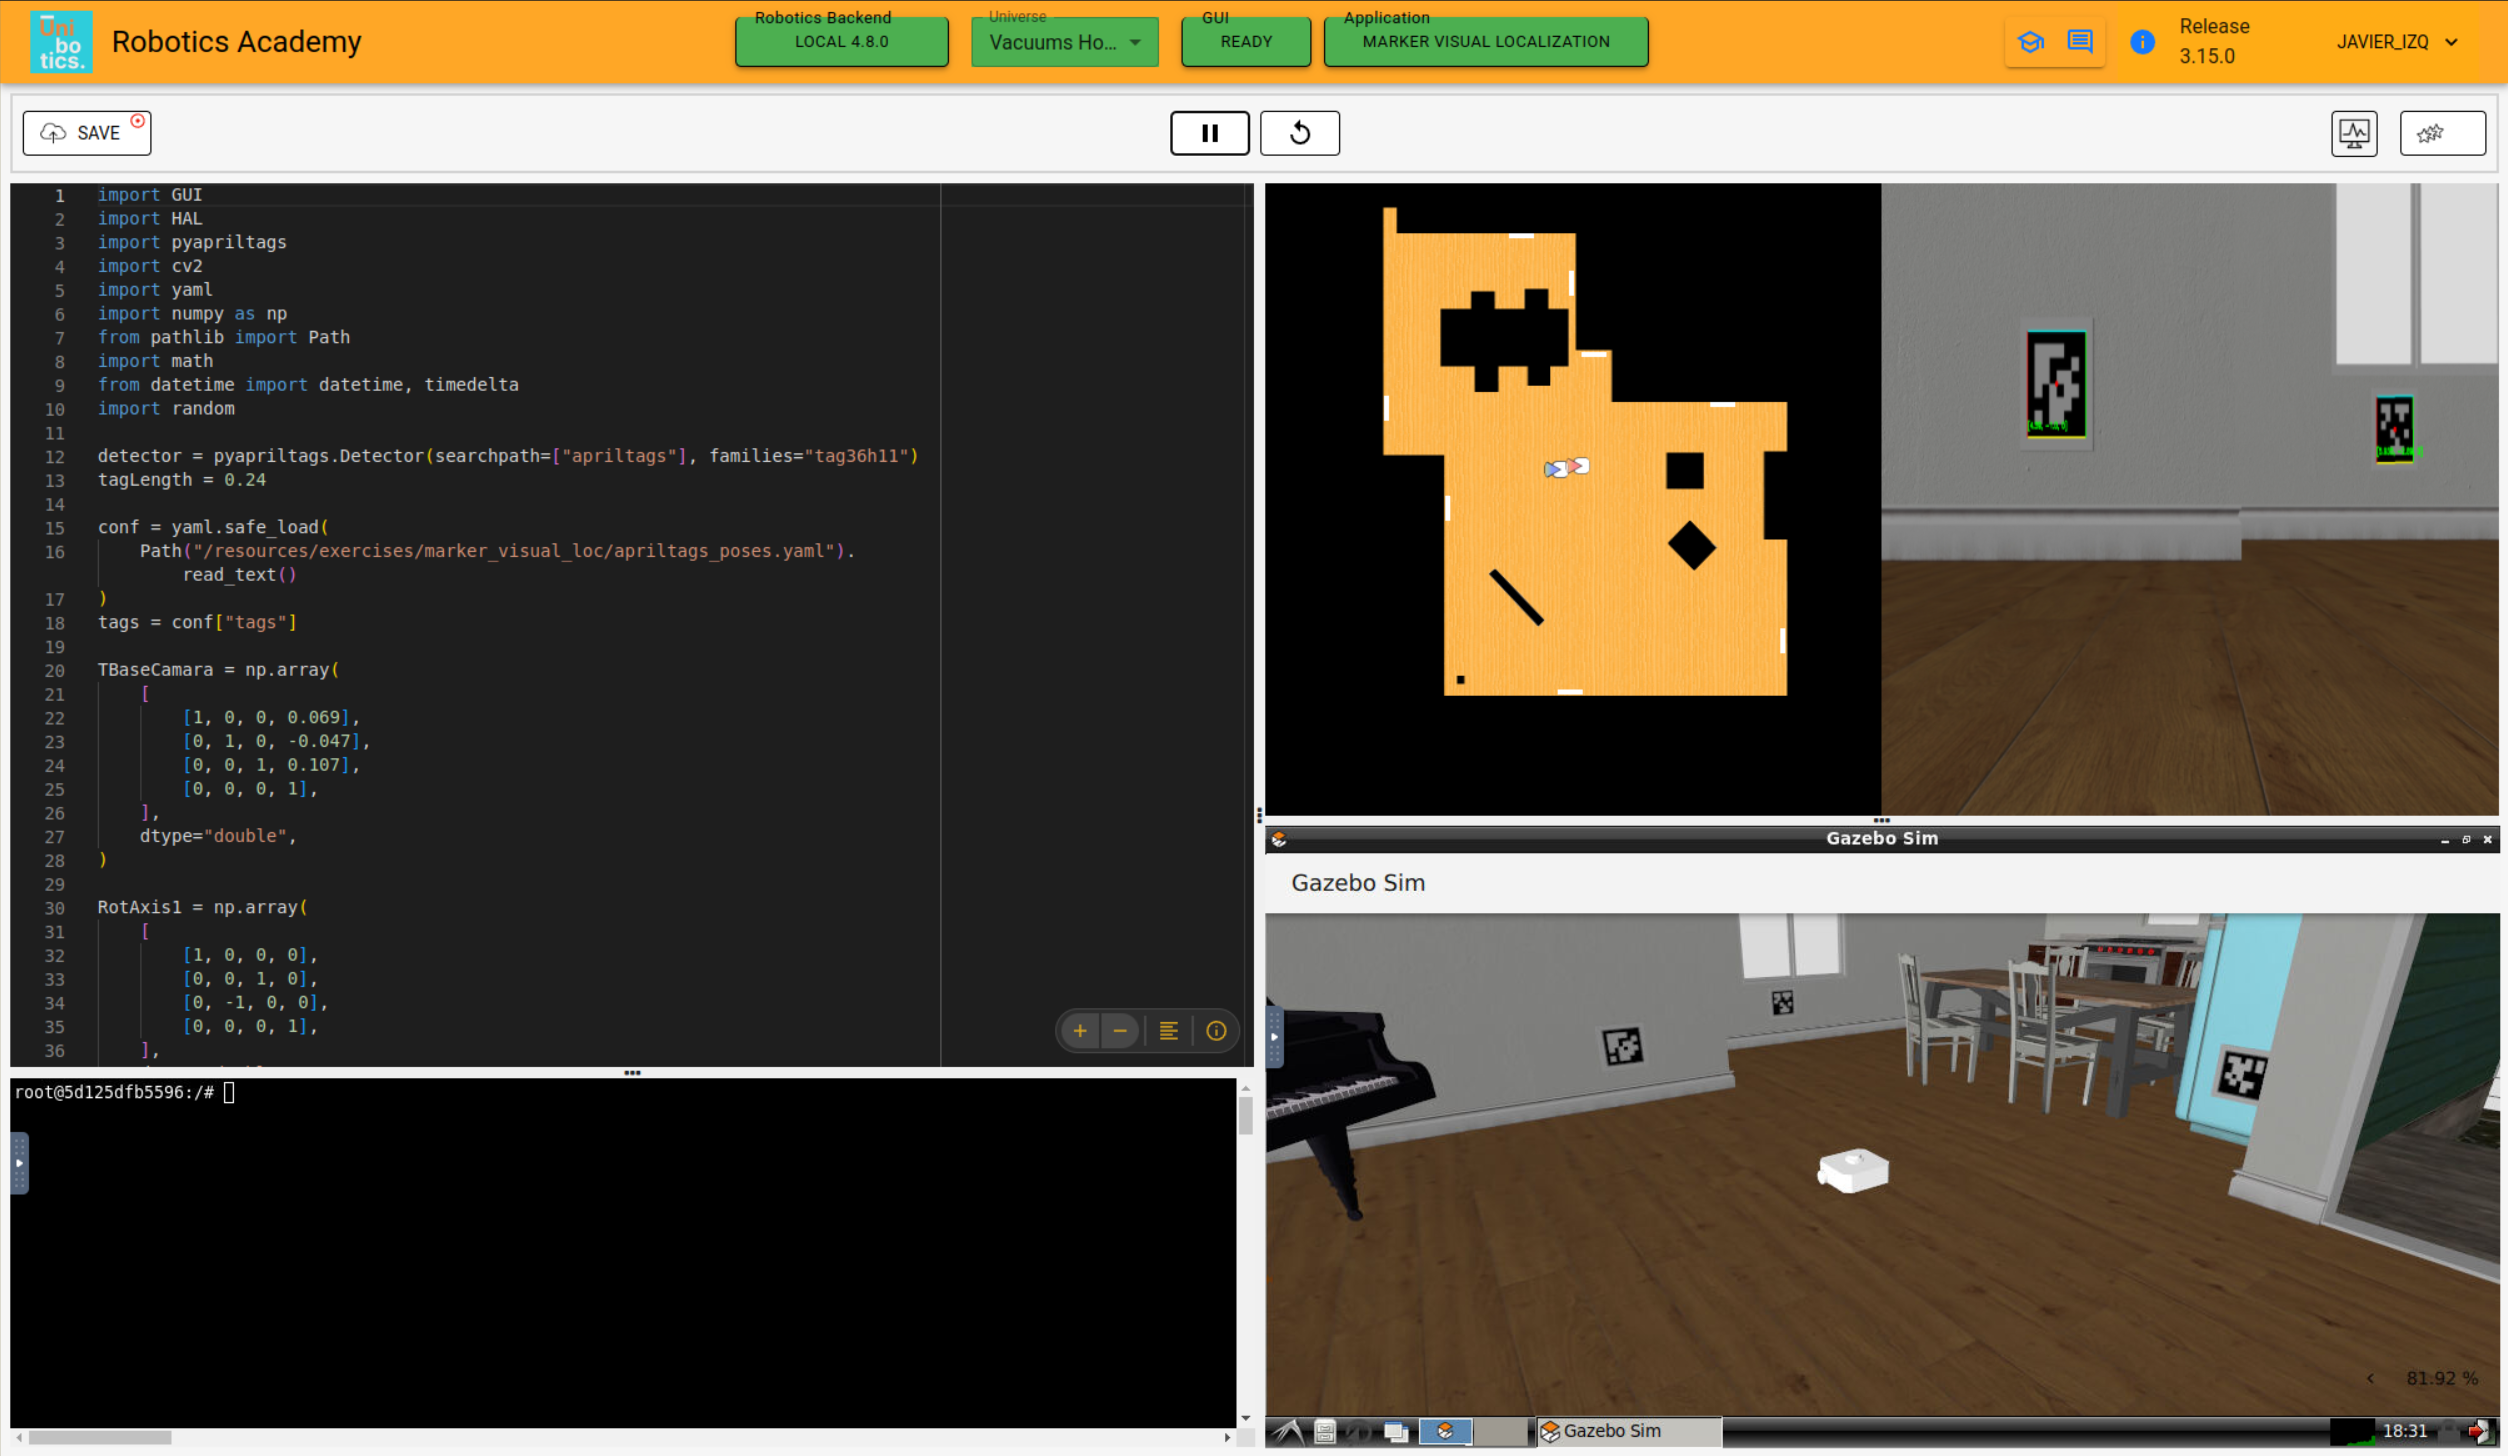
\includegraphics[width=1.0\textwidth]{figures/fundamentos/unib-demo.png}
    \caption{Aplicación robótica básica ejecutando en Unibotics}
    \label{fig:ejemplo}
\end{figure}

Por último, Unibotics, al igual que Robotics Academy, utiliza las bases de datos de universos encontradas en Robotics Infrastructure\footnote{\url{https://github.com/JdeRobot/RoboticsInfrastructure}} que han sido creadas durante este TFG.

Como se ha explicado en los objetivos de este trabajo, la integración en Unibotics es fundamental para el desarrollo y la conclusión de este. 

\subsection{Robotics Backend}\label{sec:robotics-backend}

Robotics Backend\footnote{\url{https://hub.docker.com/r/jderobot/robotics-backend}} es una imagen docker basada en Ubuntu 22.04 que permite lanzar un contenedor con un entorno de desarrollo ROS 2 completo junto con diversas herramientas adicionales. Dentro de este contenedor existe una amplia colección de universos para el simulador Gazebo con sus correspondientes \textit{launchers}.

Para manejar el uso de estas herramientas, se ejecuta dentro de este un programa gestor, llamado \textit{Robotics Application Manager} (RAM). Este es capaz de lanzar universos, preparar las distintas visualizaciones usando visores de VNC y de controlar la ejecución de aplicaciones robóticas. Desde el frontend de la aplicación, ya sea Unibotics, Robotics Academy o BT Studio, que corre en el navegador web, se comunica con el RAM usando websockets para ejecutar las acciones deseadas por estos.

Durante este TFG se ha modificado activamente el contenido del Robotics Backend, ya sea añadiendo soporte para las aplicaciones de BT Studio, los universos personalizados y la funcionalidad extra para el editor de texto en \textit{Robotics Application Manager}, o añadiendo las bases de datos de universos y migrando estos a Gazebo Harmonic en Robotics Infrastructure. 

\subsubsection{Herramientas incluidas en el Robotics Backend}

Las herramientas incluidas dentro del entorno de desarrollo son las siguientes:

\begin{enumerate}
    \item \textbf{ROS2 Humble:}
    \begin{itemize}
        \item Simulador Gazebo Classic.
        \item Simulador Gazebo Harmonic.
        \item RViz2.
    \end{itemize}
    \item \textbf{Python 3.10:}
    \begin{itemize}
        \item websocket\_server.
        \item websockets.
        \item asyncio.
    \end{itemize}
    \item \textbf{Xvfb:} xserver virtual. 
    \item \textbf{Aceleración GPU:} VirtualGL.
    \item \textbf{Servidores VNC:}
    \begin{itemize}
        \item TurboVNC.
        \item noVNC.
    \end{itemize}
    \item \textbf{Dependencias habituales de aplicaciones robóticas:}
    \begin{itemize}
        \item OpenCV.
        \item OMPL.
        \item PyTorch.
        \item TensorFlow.
        \item MoveIt.
        \item AeroStack2.
    \end{itemize}
    \item \textbf{RoboticsInfrastructure}.
    \item \textbf{RoboticsApplicationManager}.
\end{enumerate}
